%% -*- Lecture -*-

\documentclass[11pt,aspectratio=169]{beamer}

\usepackage{rcstalk}
\usetheme{rcstheme}
\usepackage{drawstack} %% TikZ based stack diagram

\topic{Threads}
\title{CS350: Operating Systems}
\subtitle{Lecture 3: Threads}

\begin{document}

\maketitle

\tikzstyle{osbox}=[draw, fill=blue!20, text width=20em, text centered, minimum 
height=2em]
\tikzstyle{osbigbox}=[draw, fill=blue!20, text width=25em, text centered, 
minimum height=5em]
\tikzstyle{apibox}=[draw, fill=white, text width=5em, text centered, minimum 
height=2em]
\tikzstyle{hwbox}=[draw, fill=green!20, text width=20em, text centered, minimum 
height=2em]
\tikzstyle{appbox}=[draw, fill=white, text width=5em, text centered, minimum 
height=2em]
\def\blockdist{0.5}

\begin{slide}{Today: Threads}
\begin{figure}[ht!]
\centering
\begin{tikzpicture}
    \node (os) [osbigbox] {Operating System};
    \path (os.south)+(0,-\blockdist) node (hw) [hwbox] {Hardware: CPU, Memory
    and Devices};
    \path (os.north)+(0,2*\blockdist) node (emacs) [appbox,fill=yellow!30,text
    width=20em] {emacs};
    \path (os.north)+(-9em,0.1) node (procs) [apibox] {Process};
    \path (procs.east)+(1.25,0) node (threads) [apibox,fill=red!20] {Threads};
    \path (threads.east)+(1.25,0) node (locks) [apibox] {Locks};
    \path (locks.east)+(1.25,0) node (etc) [apibox] {File I/O};
\end{tikzpicture}
\end{figure}
\end{slide}

\section{Threads}

\begin{slide}{Threads}
\centerline{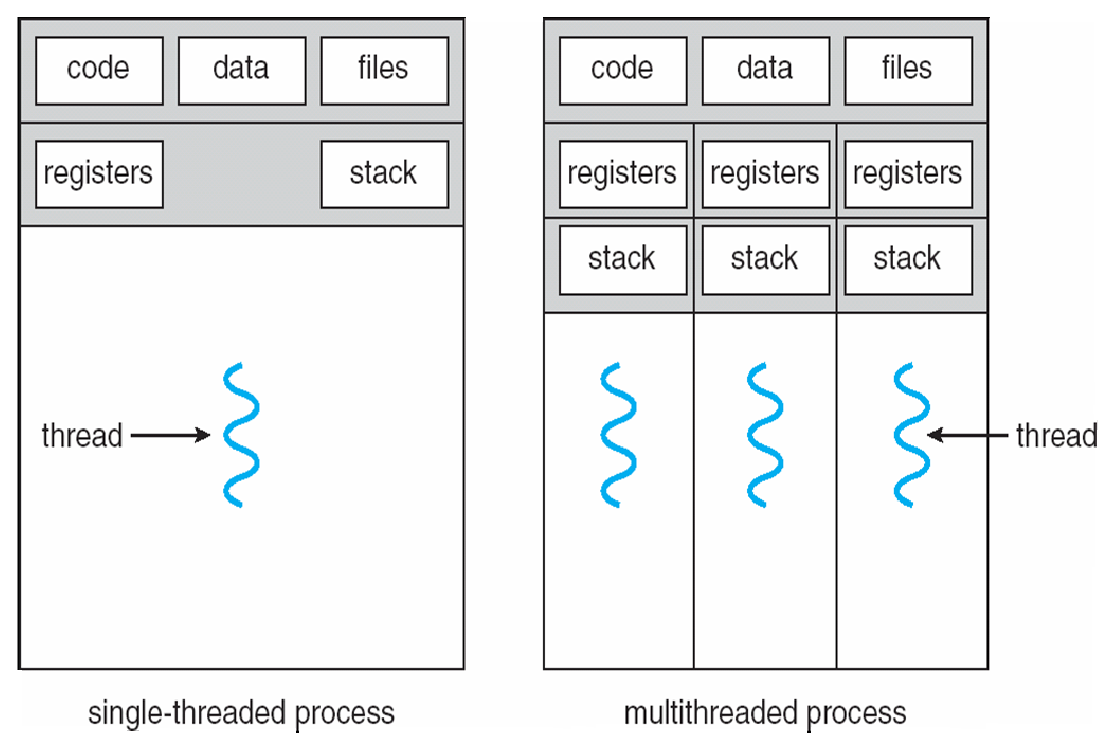
\includegraphics[height=53mm]{figs/thread}}
\itms{
  \item A thread is a schedulable execution context
  \ittms{
    \item Program counter, registers, stack (local variables) \ldots
  }
  \item Multi-threaded programs share the address space (global variables, heap, \ldots)
}
\end{slide}

\begin{slide}{Why threads?}
\itms{
  \item Most popular abstraction for concurrency
  \ittms{
    \item Lighter-weight abstraction than processes
    \item All threads in one process share memory, file descriptors, etc.
  }
  \item Allows one process to use multiple CPUs or cores
  \item Allows program to overlap I/O and computation
  \ittms{
    \item Same benefit as OS running \texttt{emacs} \& \texttt{gcc}
	    simultaneously
    \item E.g., threaded web server services clients simultaneously:
  }
}
\vspace*{-1ex}
\begin{ccode}
        for (;;) {
          fd = accept_client ();
          thread_create (service_client, &fd);
        }
\end{ccode}
\itms{
  \item Most kernels have threads, too
  \ittms{
    \item Typically at least one kernel thread for every process
  }
}
\end{slide}


\begin{slide}{POSIX thread API}
\itms{
  \item \texttt{int \man{pthread\_create}(pthread\_t *thr, pthread\_attr\_t *attr,\\
				     \hspace{11em}void *(*fn)(void *), void *arg);}
  \ittms{
    \item Create a new thread identified by \texttt{thr} with optional attributes, run \texttt{fn} with \texttt{arg}
  }
  \item \texttt{void \man{pthread\_exit}(void *return\_value);}
  \ittms{
    \item Destroy current thread and return a pointer
  }
  \item \texttt{int \man{pthread\_join}(pthread\_t thread, void **return\_value);}
  \ittms{
    \item Wait for thread \texttt{thread} to exit and receive the return value
  }
  \item \texttt{void \man{pthread\_yield}();}
  \ittms{
    \item Tell the OS scheduler to run another thread or process
  }
  \item Plus lots of support for synchronization (next Lecture and see \cref{readings/birrell.pdf}{[Birell]})
}
\end{slide}


\begin{slide}{Kernel threads}

\centerline{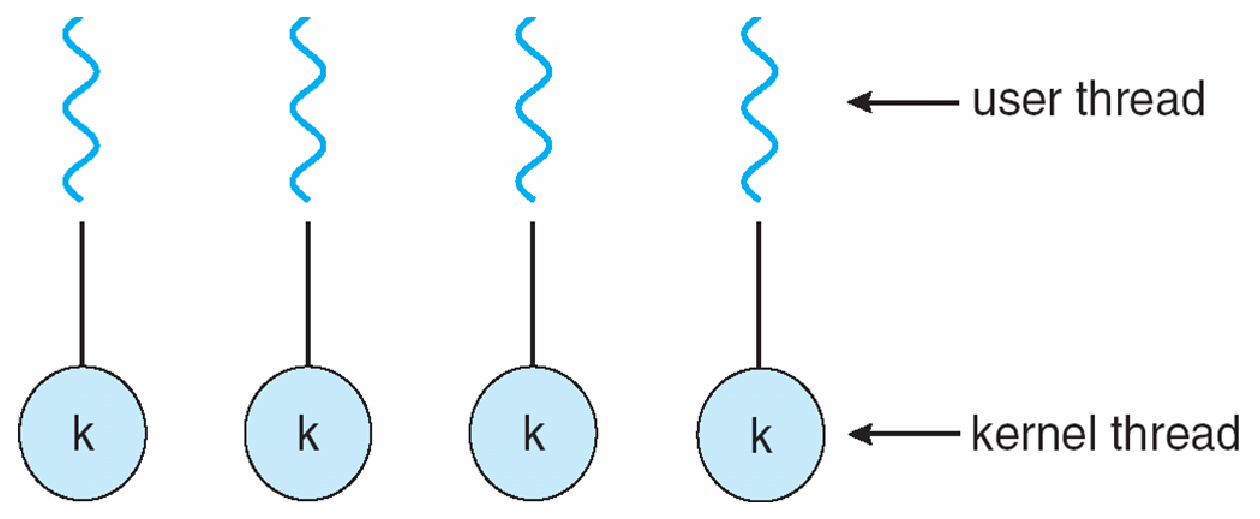
\includegraphics[height=32mm]{figs/kthread}}

\itms{
  \item Can implement \texttt{pthread\_create} as a system call
  \item To add \texttt{pthread\_create} to an OS:
  \ittms{
    \item Start with process abstraction in kernel
    \item \texttt{pthread\_create} like process creation with features
      stripped out
    \itttms{
      \item Keep same address space, file table, etc., in new process
      \item \man{rfork}/\texttt{clone} syscalls actually allow individual 
	  control
    }
  }
  \item Faster than a process, but still very heavy weight
}
\end{slide}

\begin{slide}{Limitations of kernel-level threads}
\itms{
  \item Every thread operation must go through kernel
  \ittms{
    \item create, exit, join, synchronize, or switch for any reason
    \item Syscall takes 100 cycles, function call 2 cycles
    \item Result: threads 10$\times$--30$\times$ slower when implemented in kernel
    \item Worse today because of \cref{readings/spectre.pdf}{SPECTRE}/\cref{readings/meltdown.pdf}{Meltdown} mitigations
  }
  \item One-size fits all thread implementation
  \ittms{
    \item Kernel threads must please all people
    \item Maybe pay for fancy features (priority, etc.) you don't need
  }
  \item General heavy-weight memory requirements
  \ittms{
    \item E.g., requires a fixed-size stack within kernel
    \item Other data structures designed for heavier-weight processes
  }
}
\end{slide}

\begin{slide}{User threads}
\centerline{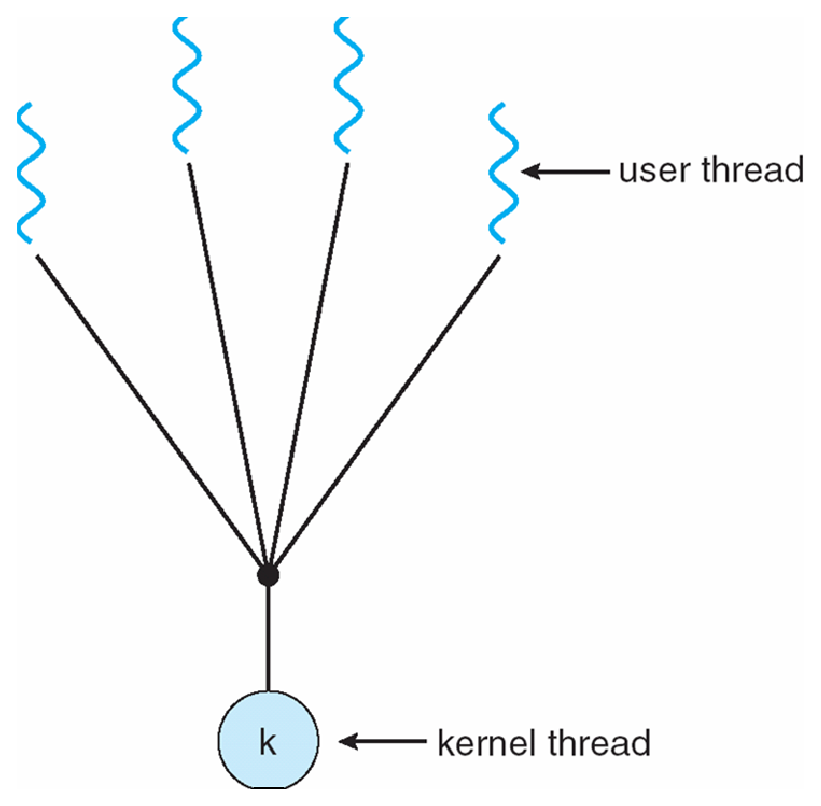
\includegraphics[height=50mm]{figs/uthread}}
\itms{
  \item An alternative: implement in user-level library
  \ittms{
    \item One kernel thread per process
    \item \texttt{pthread\_create}, \texttt{pthread\_exit}, etc., just library functions
  }
}
\end{slide}

\begin{slide}{Implementing user-level threads}
\itms{
  \item Allocate a new stack for each \man{pthread\_create}
  \item Keep a queue of runnable threads
  \item Replace blocking system calls (\texttt{read}/\texttt{write}/etc.)
  \ittms{
    \item If operation would block, switch and run different thread
  }
  \item Schedule periodic timer signal (\man{setitimer})
  \ittms{
    \item Switch to another thread on timer signals (preemption)
  }
  \item Multi-threaded web server example
  \ittms{
    \item Thread calls \texttt{read} to get data from remote web browser
    \item ``Fake'' \texttt{read} \emph{function} makes \texttt{read}
      \emph{syscall} in non-blocking mode
    \item No data?  schedule another thread
    \item On timer or when idle check which connections have new data
  }
  %\item How to switch threads?
}
\end{slide}

\begin{slide}{Limitations of user-level threads}
\itms{
  \item Can't take advantage of multiple CPUs or cores
  \item A blocking system call blocks all threads
  \ittms{
    \item Can replace \texttt{read} to handle network connections
    \item But usually OSes don't let you do this for disk
    \item So one uncached disk read blocks all threads
  }
  \item A page fault blocks all threads
  \item Possible deadlock if one thread blocks on another
  \ittms{
    \item May block entire process and make no progress
    \item {}[More on deadlock in future lectures.]
  }
}
\end{slide}

\begin{slide}{User threads on kernel threads}
\centerline{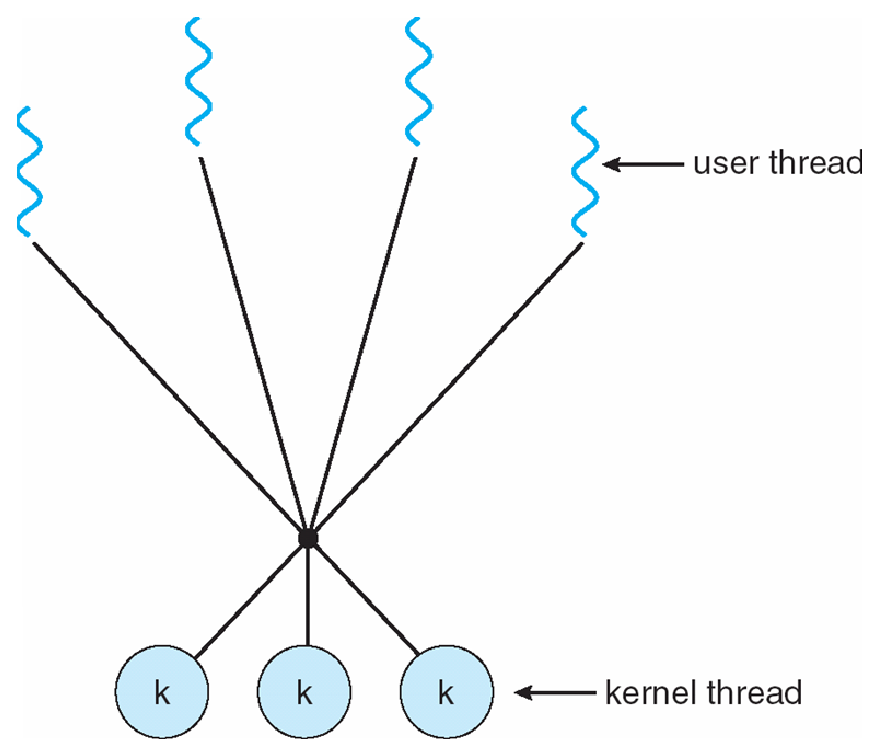
\includegraphics[height=1.6in]{figs/ukthread}}
\itms{
  \item User threads implemented on kernel threads
  \ittms{
    \item Multiple kernel-level threads per process
    \item \texttt{thread\_create}, \texttt{thread\_exit}
      still library functions as before
  }
  \item Sometimes called $n:m$ threading
  \ittms{
    \item Have $n$ user threads per $m$ kernel threads \\
      (Simple user-level threads are $n:1$, kernel threads $1:1$)
  }
}
\end{slide}

\begin{slide}{Limitations of $n:m$ threading}
\vspace{-1em}
\begin{columns}
\column{0.7\textwidth}
\itms{
  \item Many of same problems as $n:1$ threads
  \ittms{
    \item Blocked threads, deadlock, \ldots
  }
  \gap
  \item Hard to keep same \# kthreads as available CPUs
  \ittms{
    \item Kernel knows how many CPUs available
    \item Kernel knows which kernel-level threads are blocked
    \item Tries to hide these things from applications for
      transparency
    \item User-level thread scheduler might think a thread is
      running while underlying kernel thread is blocked
  }
  \gap
  \item Kernel doesn't know relative importance of threads
  \ittms{
    \item Might preempt kthread in which library holds important lock
  }
}
\column{0.3\textwidth}
\end{columns}
\end{slide}

\begin{slide}{Lessons}
\itms{
  \item Threads best implemented as a library
  \ittms{
    \item But kernel threads not best interface on which to do this
  }
  \item Better kernel interfaces have been suggested
  \ittms{
    \item See Scheduler Activations
\href{http://www.cs.washington.edu/homes/tom/pubs/sched_act.pdf}{[Anderson et al.]}
    \item Maybe too complex to implement on
      existing OSes (some have added then removed such features, now
      Windows is trying it)
  }
  \item Today shouldn't dissuade you from using threads
  \ittms{
    \item Standard user or kernel threads are fine for most purposes
    \item Use kernel threads if I/O concurrency main goal
    \item Use $n:m$ threads for highly concurrent (e.g,. scientific
 applications) with many thread switches
  }
  \item \ldots though concurrency/synchronization lectures may
  \ittms{
    \item Concurrency greatly increases the complexity of a program!
    \item Leads to all kinds of nasty race conditions
  }
}
\end{slide}

\section{Case Study: Go Language and Runtime}

\begin{slide}{Go Routines}
\itms{
  \item Go routines are very light-weight
  \ittms{
    \item Running 100k go routines is practical
    \item Custom compiler enables stack segmentation, preemption, and garbage collection
    \item Runs on segmented stack -- stack allocated on demand to avoid memory use
    \item OS thread typically allocate 2~MiB fixed stacks
  }
  \gap
  \item Go routines on top of Kernel threads (n:m Model)
  \ittms{
    \item Multi-core scalability and efficient user-level threads
    \item One pthread (kernel-level thread) per CPU core
    \item Supports many user-level threads as you like
  }
}
\end{slide}

\begin{slide}{Go Routine Continued}
\itms{
  \item Each kernel-level thread finds and runs a go routine (user-level thread)
  \gap
  \item Every logical core is owned by a kernel thread when running
  \gap
  \item Convert blocking system calls (when possible):
  \ittms{
    \item Converted to non-blocking by in the runtime yielding the CPU to another core
    \item Cores poll using kernel event API \man{poll}, {\tt epoll}, or 
	\man{kqueue}
  }
  \item Blocking system calls:
  \ittms{
    \item Release the "CPU" to another kernel-level thread before the call
    \item Let the kernel thread sleep
    \item Regain the "CPU" thread when done
  }
}
\end{slide}

\begin{slide}{Go Channels}
\itms{
  \item Go routine communicate and synchronize through {\em channels} 
}
\begin{ccode}[language=Go]
func worker(done chan bool) {
    // Notify the main routine
    done <- true
}

func main() {
    // Create a channel to notify us
    done := make(chan bool, 1)

    // Create go routine
    go worker(done)

    // Block until we receive a message
    <-done
}
\end{ccode}
\end{slide}

\section{How to implement threads in COS}

\begin{slide}{Background: AMD64/x86-64 calling conventions}
  \vspace{-1em}
  \begin{columns}
  \column{.65\textwidth}   
  \itms{
    \item Registers divided into 2 groups
    \ittms{
      \item Functions free to clobber \Red{\emph{caller-saved}}
	\rlap{regs} \\
	(\texttt{\%r10}, \texttt{\%r11}, arguments and return registers)
      \item But must restore \Red{\emph{callee-saved}} ones to
	  original value upon return (\texttt{\%rbx}, 
	  \texttt{\%r12}--\texttt{\%r15})
      }
    \item \texttt{\%rsp} register always base of stack
    \ittms{
    \item Frame pointer (or base pointer) (\texttt{\%rbp}) is old 
	\texttt{\%rsp}
    }
    \item Local variables stored in registers and on stack
    \item Function arguments go in caller-saved regs and on stack
    \ittms{
    \item First six arguments in \texttt{\%rdi}, \texttt{\%rsi}, 
	\texttt{\%rdx}, \texttt{\%rcx}, \texttt{\%r8}, \texttt{\%r9}
      \item Remaining arguments on stack
    }
    \item Return value \texttt{\%rax} and \texttt{\%rdx}
  }
  \column{.05\textwidth}
  \column{.3\textwidth}
  \input{stkframe.tex}
  \end{columns}
\end{slide}

\begin{slide}{Background: procedure calls}
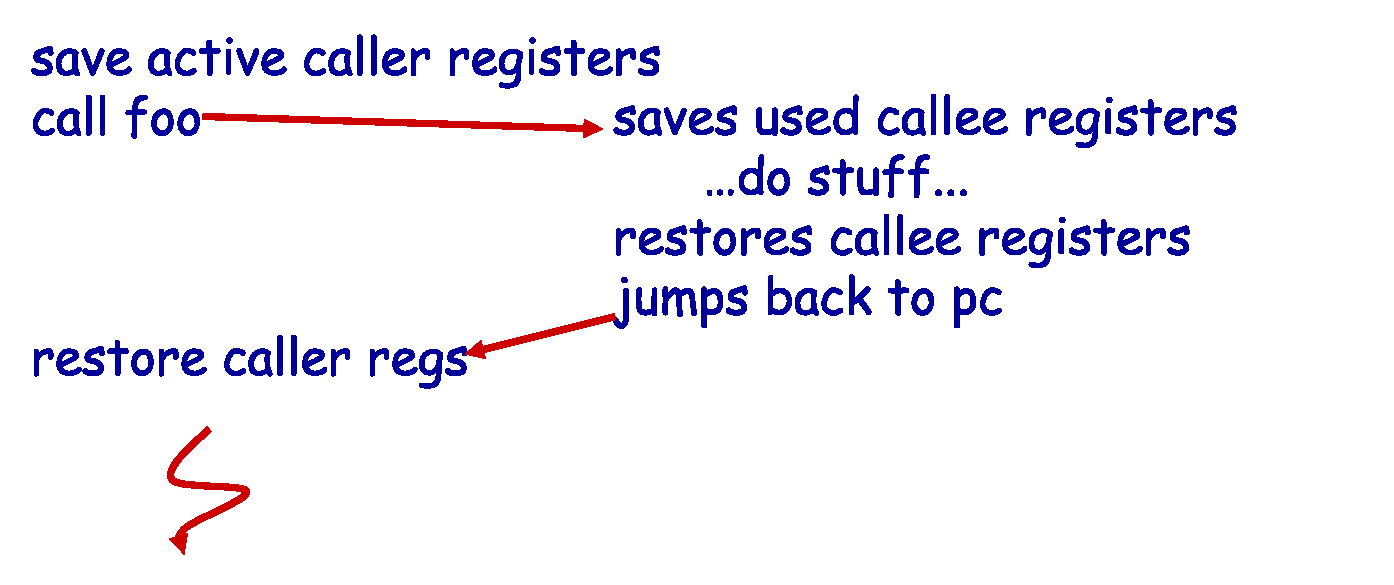
\includegraphics[height=48mm]{figs/proc}
\itms{
  \item Some state saved on stack
  \ittms{
    \item Return address, caller-saved registers
  }
  \item Some state not saved
  \ittms{
    \item Callee-saved regs, global variables, stack pointer
  }
}
\end{slide}

\begin{slide}{Threads vs.\ procedures}
\itms{
\item Threads may resume out of order: 
\ittms{
  \item Cannot use LIFO stack to save state
  \item General solution: one stack per thread
}
\item Threads switch less often:
\ittms{
  \item Don't partition registers (why?)
}
\item Threads can be involuntarily interrupted:
\ittms{
  \item Synchronous: procedure call can use compiler to save state
  \item Asynchronous: thread switch code saves all registers
}
\item More than one than one thread can run at a time:
\ittms{
  \item Procedure call scheduling obvious: Run called procedure
  \item Thread scheduling: What to run next and on which CPU?  
}
}
\end{slide}

\begin{slide}{User-level Threading}
\itms{
  \item POSIX even included some helper functions to help you build user-level 
      threads.
  \item \texttt{void \man{makecontext}(ucontext\_t *ucp, void (*func)(void),}\\
      \hspace{10em}\texttt{int argc, ...);}
  \ittms{
    \item Modify a previously created context with a function pointer and args
    \item Use \texttt{getcontext} to create a valid context, then allocate a 
	stack
  }
  \item \texttt{int \man{swapcontext}(ucontext\_t *old, ucontext\_t *new);}
  \ittms{
    \item Save the current thread into \texttt{old}, restore the \texttt{new} 
	thread
    \item Saves and restores all CPU registers including the stack pointer
  }
  \item \texttt{int \man{getcontext}(ucontext\_t *ucp);}
  \ittms{
    \item Get the current thread context and save it in \texttt{ucp}
  }
}
\end{slide}

\begin{slide}{User-level Threading: Creating a Fiber}
\begin{ccode}
ucontext_t ctx;

// Use the current thread to initialize ctx to a valid state
// Why? Some CPU registers (e.g., rflags) require specific values
getcontext(&ctx);

// Allocate a stack
ctx.uc_stack.ss_sp = malloc(SIGSTKSZ);
ctx.uc_stack.ss_size = SIGSTKSZ;

// uc_link says what to do when done, NULL terminates the program.
ctx.uc_link = NULL;

// Initialize the context pointing to the function foo
makecontext(&ctx, (void (*)())foo, 0);
\end{ccode}
\end{slide}

\begin{slide}{User-level Threading: Context Switching}
\itms{
\item \texttt{swapcontext}: Saves and Restores the CPU state \& swaps stacks
\item \texttt{ucontext\_t}: Contains all CPU state
}
\vspace{1em}

\begin{tikzpicture}[every node/.style={scale=0.5,font=\sffamily}, scale=0.5]
\node (core) [] {\texttt{swapcontext()}};
\path (core)+(-8, -3) node (thr1) [draw, text width=6em, minimum height=4em, 
    drop shadow] {\texttt{ucontext\_t}};
\path (core)+(8, -3) node (thr2) [draw, text width=6em, minimum height=4em, 
    drop shadow] {\texttt{ucontext\_t}};
\path [draw, ->] (core) -- node [above] {Save CPU State} (thr1);
\path [draw, ->] (thr2) -- node [above] {Restore CPU State} (core);
\end{tikzpicture}

\vspace{1em}

\begin{columns}
\column{0.5\textwidth}
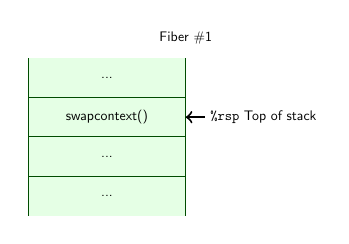
\begin{tikzpicture}[every node/.style={scale=0.5,font=\sffamily}, scale=0.5]
\node[] at (2, 1) (stk1) {Fiber \#1};
\stacktop{}
    \cell{swapcontext()} \cellptr{\texttt{\%rsp} Top of stack}
    \cell{...}
\stackbottom
\end{tikzpicture}

\column{0.5\textwidth}
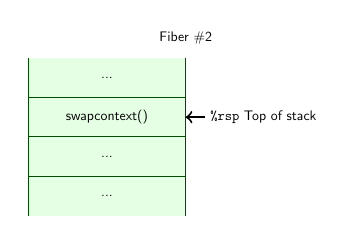
\begin{tikzpicture}[every node/.style={scale=0.5,font=\sffamily}, scale=0.5]
\node[] at (2, 1) (stk2) {Fiber \#2};
\stacktop{}
    \cell{swapcontext()} \cellptr{\texttt{\%rsp} Top of stack}
    \cell{...}
\stackbottom
\end{tikzpicture}
\end{columns}

\end{slide}

\begin{slide}{COS: Thread Details}
  \itms{
    \item Supports both kernel and user threads
    \item Basic Pthreads support see lib/libc/posix/pthread.c
    \item Mechanically similar to the fiber example
  }
  \gap

\begin{ccode}
/* Create a kernel thread associated with the process */
Thread *Thread_KThreadCreate(void (*f)(void *), void *arg);

/* Create a userspace thread (and associated kernel thread */
Thread *Thread_UThreadCreate(Thread *oldThr,
				       uint64_t rip,
				       uint64_t arg);
\end{ccode}
\end{slide}


\begin{slide}{COS: Switching Threads}
  \itms{
    \item All thread switches go through \code{Sched_Scheduler()} and 
	\code{Sched_Switch()}
    \item \code{Sched_Switch()} calls \code{Thread_SwitchArch()} that runs 
	\code{switchstack}
    \item \code{switchstack} switches from one stack to other while saving and 
	restoring registers
    \gap
  }

\begin{columns}
  \column{0.5\textwidth}
  \centering
  General (from Kernel)\\
  \column{0.5\textwidth}
  \centering
  Hardware Interrupt (typically Timer)\\
\end{columns}
\vspace{1em}
\begin{columns}
  \column{0.5\textwidth}
  \centering
    \begin{drawstack}[every node/.style={scale=0.5,font=\sffamily}, scale=0.5]
	\cell{Sched\_Scheduler()}
    \cell{Sched\_Switch()}
    \cell{Thread\_SwitchArch()}
    \cell{switchstack()}
    \cell{switchframe}
  \end{drawstack}
  \column{0.5\textwidth}
  \centering
    \begin{drawstack}[every node/.style={scale=0.5,font=\sffamily},scale=0.5]
    \cell{struct Trapframe}
    \cell{trap\_entry()}
    \cell{interrupt handler ...}
    \cell{Thread\_SwitchArch()}
    \cell{switchstack()}
    \cell{struct switchframe}
  \end{drawstack}
\end{columns}
\end{slide}

\begin{slide}{COS: switchstack -- switch kernel threads}
From COS kern/amd64/switch.S
\begin{columns}
\column{0.9\textwidth}
\begin{asm}[numbers=left,firstnumber=9]
# switch(uint64_t *oldsp, uint64_t newsp)
# %rdi: oldsp
# %rsi: newsp
FUNC_BEGIN(switchstack)
    # Save callee saved registers of old thread
    pushq   %rbp
    pushq   %rdi
    pushq   %rbx
    pushq   %r12
    pushq   %r13
    pushq   %r14
    pushq   %r15

    # Switch stack from old to new thread
    movq    %rsp, (%rdi)
    movq    %rsi, %rsp
\end{asm}
\end{columns}
\end{slide}

\begin{slide}{COS: switchstack -- switch kernel threads (con't)}
  \vspace{-1.7em}
  \begin{columns}
  \column{0.9\textwidth}
  \begin{asm}[numbers=left, firstnumber=25]

    # Restore callee saved registers of new thread
    popq    %r15
    popq    %r14
    popq    %r13
    popq    %r12
    popq    %rbx
    popq    %rdi
    popq    %rbp
    ret
FUNC_END(switchstack)
  \end{asm}
\end{columns}
\end{slide}

\end{document}
